
\chapter{Generativni modeli}

U ovom poglavlju pogledat ćemo jedan drugačiji pristup učenju. Tehnike i arhitekture s kojima smo se do sada bavili mogli bismo okarakterizirati kao \textbf{diskriminativne} - cilj nam je bio povezati uzorke skupa za učenje sa odgovarajućim oznakama (klasa slike, oznake piksela itd.) S druge strane, \textbf{generativni} pristup nastoji što točnije naučiti distribuciju podataka za učenje, kako bi na osnovu njih mogao generirati nove podatke iz te distribucije. Primijetimo da rezultati ova dva pristupa mogu biti identični, no način na koji dolazimo do rezultata je fundamentalno različit. Za određene primjene, generativni modeli su se u praksi pokazali kao puno bolji izbor od diskriminativnih.

Malo formalnije, ako imamo zadan skup ulaznih podataka X te set očekivanih izlaza Y, diskriminativni modeli pokušavaju naučiti uvjetnu vjerojatnost $P(Y|X)$. Dakle, diskriminativne modele ne zanima koja je vjerojatnost pojave takvog para, nego samo što će biti s izlazom Y ako se na ulazu pojavi X. S druge strane, generativni modeli uče vjerojatnost $P(X,Y)$, odnosno mogu naučiti koja je vjerojatnost pojave konkretnog ulaza X i ulaza Y u isto vrijeme. Dakle oni uče i koja je vjerojatnost pojave određene kombinacije ulaza i izlaza

Konačno, pogledajmo razliku u pristupima diskriminativnog i generativnog modela na jednom konkretnom primjeru, prikazan na slici 3.9. Primjer je preuzet iz \citep{generativeGoogle}

\begin{figure}[htb]
\centering
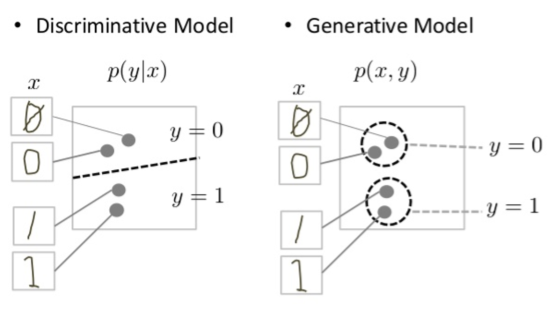
\includegraphics[width=12cm]{slike/generative_v_discriminative.png}
\caption{Diskriminativni vs generativni pristup \citep{generativeGoogle}}
\label{fig:fer-logo}
\end{figure}
\textbf{}

\noindent Razlika je objašnjenja u razlici pristupu problemu klasifikacije slika rukom napisanih znamenki, vrlo čestog primjera u području računalnog vida. Diskriminativni model nastoji odrediti razliku između dvije prikazane klase, 0 i 1, povlačenjem linije u prostoru svih podataka. Ta linija dijeli prostor na dva dijela - prostor u kojem su podaci koje je potrebno klasificirati kao 0, te prostor u koji pripadaju podaci koje je potrebno klasificirati kao 1. Ako model dobro "pogodi" poziciju te linije, može uspješno klasificirati dane ulaze u jednu od te dvije klase, bez da ikad mora naučiti koja je točna pozicija konkretnih ulaza u tom prostoru. S druge strane, generativni model nastoji naučiti točne pozicije konkretnih ulaza u prostoru podataka, dakle moraju naučiti na koji način su podaci \textbf{distribuirani} u prostoru podataka. Očito je da je to znatno složeniji pristup u odnosu na diskriminativni model, no to mu također omogućuje generiranje novih podataka iz dane distribucije.\\

\noindent U nastavku ćemo detaljnije pogledati primjere danas vrlo popularne obitelji arhitektura generativnih modela, zasnivanih na GAN arhitekturi.



\section{GAN}
\textbf{Generativna suparnička mreža} \engl{generative adversarial network, GAN} je naziv za arhitekturu dubokih generativnih modela prvi put predloženu od strane Goodfellowa i dr. u njihovom poznatom radu \citep{GoodfellowGAN}.

Autori predlažu arhitekturu koja se sastoji od 2 suparničke mreže - \textbf{generatora}, G i \textbf{diskriminatora} D. G je generativni model čija je zadaća što točnije naučiti distribuciju ulaznih podataka te generirati nove ("lažne") primjerke iz te distribucije. D je diskriminativni model čija je zadaća za dani ulaz odrediti vjerojatnost dolazi li iz skupa ulaznih (originalnih, pravih) podataka ili se radi o "lažnom" primjerku ulaza koji je G generirao. G se trenira tako da nastoji maksimizirati vjerojatnost da D napravi pogrešku, dok D treniramo tako da njegove procjene budu što točnije. Ovakav pristup odgovara igri \textbf{minimaks} sa 2 igrača, G i D, u kojoj svaki igrač nastoji maksimizirati vjerojatnost svoje pobjede i minimizirati vjerojatnost pobjede protivnika (provjeri je li ovo dobra interpretacija minimaxa!). Kako želimo da generator generira što točnije uzorke iz ciljne distribucije, konačni cilj ove igre je situacija u kojoj je G savršeno naučio ulaznu distribuciju i može generirati podatke praktički jednake onima iz ulazne distrucije, dok D za svaki ulaz daje vjerojatnost 0.5 jer ne može razaznati radi li se o originalnom ili "lažnom" podatku.

Kako bismo formalno definirali funkciju cilja ove arhitekture, uvedimo sljedeću nomenklaturu. Neka nam $x$ predstavlja određeni ulazni podatak (primjerice 2D sliku). Sa $D(x)$ ćemo označiti diskriminatorsku mrežu koja za dani ulaz $x$ vraća skalar - vjerojatnost da $x$ dolazi iz podataka za treniranje, a ne iz generatora. Ukoliko $x$ dolazi iz podataka za treniranje, očekujemo da će izlaz $D(x)$ biti velik, dok za slučaj kad je $x$ izlaz generatora očekujemo da će $D(x)$ biti malen. $D(x)$ se dakle ponaša kao običan binarni klasifikator. Nadalje, sa $z$ označimo slučajni vektor iz normalne distribucije. $G(z)$ će onda biti generatorska funkcija koja mapira $z$ na prostor ulaznih podataka. Kao što smo već rekli, cilj $G(z)$ je što točnije naučiti distribuciju ulaznih podataka kako bi to mapiranje bilo što točnije. Iz navedenog slijedi da sa $D(G(z))$ možemo označiti vjerojatnost s kojom je  $D(x)$ siguran da izlaz generatora $G(z)$ dolazi iz originalnog skupa podataka. Konačno, funkciju cilja ove arhitekture možemo definirati kao: 

\NewEnviron{myequation}{%
    \begin{equation}
    \scalebox{1}{$\BODY$}
    \end{equation}
    }

\begin{myequation}%
\bm{\mathop{min}\limits_{G}\mathop{max}\limits_{d}V(D,G) = \mathbb{E}_{x \sim p_{data}(x) } [logD(x)] + \mathbb{E}_{x \sim p_{z}(z)}[log(1-D(G(z)))]
}  %
\end{myequation}

\noindent gdje $\mathbb{E}_{x \sim p_{data}(x) }$ predstavlja očekivanu vrijednost nad svim pravim ulazima, a $\mathbb{E}_{x \sim p_{z}(z)}$ očekivanu vrijednost nad svim lažnim (generiranim) ulazima. D nastoji maksimizirati $logD(x)$, vjerojatnost da će uspješno klasificirati ulazne podatke. G nastoji minimizirati vjerojatnost $(log(1-D(G(z)))$, odnosno da će D ispravno klasificirati njegove izlaze kao lažne.

Autori također navode da u ranim fazama treniranja, dok generator još nije dobro naučio ciljnu distribuciju ulaza, D može raspoznavati prave od lažnih ulaza s vrlo visokom točnosti, što može dovesti do zasićenja $log(1 − D(G(z)))$, odnosno do toga da GAN "zapne" prilikom treniranja. Kao alternativu možemo trenirati G da maksimizira $log D(G(z))$ umjesto da minimizira $log(1 − D(G(z)))$. Ovo u osnovi predstavlja istu ideju, samo što ovaj rezultira puno strmijim gradijentima u ranoj fazi treniranja.\\


\noindent Treniranje GAN-a je zahtijevnije od treniranja ostalih dubokih modela iz dva razloga: 

\begin{enumerate}[label=(\alph*)]
\item Moramo uspješno trenirati 2 mreže: generator i diskriminator
\item Konvergenciju GAN-a je teško definirati, a time i otkriti
\end{enumerate}

Stoga GAN-ove obično treniramo na tako da prvo fiksiramo parametre generatora i treniramo diskriminator jednu ili više epoha. Ovo je potrebno jer u suštini diskriminator treniramo da prepozna mane u generatoru; kad bi istovremeno mijenjali diskriminator i generator, to bi bio gotovo nemoguć problem. Slično u sljedećem koraku: fiksiramo parametre diskriminatora te treniramo generator. Također, bitno je treniranje zaustaviti na vrijeme, obično kada diskriminator više ne može razlikovati prave ulaze od lažnih. Ako nastavimo trenirati nakon te točke, generator se trenira na pogrešnim povratnim informacijama od diskriminatora, te može doći do pogoršanja njegovih performansi. \\

\noindent Puni algoritam za treniranje dajem u nastavku.

\begin{algorithm}
  \caption{Algoritam treniranja generativnih suparničkih mreža}
  \begin{algorithmic}
      \For{broj iteracija}
        \For{k koraka}
            \begin{itemize}
              \item Uzmi m slučajnih uzoraka šuma ${(z^{(1)}...z^{(m)})}$
              \item Uzmi m ulaznih primjera ${(x^{(1)}...x^{(m)})}$ iz skupa ulaznih podataka
              \item Ažuriraj diskriminator penjući se njegovim stohastičkim gradijentom: 
              $$\nabla_{ \Theta _{d}} \cdot\frac{1}{m}  \sum\limits_{i=1}^m [log D(x^{(i)} + log(1-D(G(z^{(i)})))]$$
            \end{itemize}
        \EndFor
            \begin{itemize}
              \item Uzmi m slučajnih uzoraka šuma ${(z^{(1)}...z^{(m)})}$
              \item Ažuriraj generator spuštajući se njegovim stohastičkim gradijentom: 
              $$\nabla_{ \Theta _{g}} \cdot\frac{1}{m}  \sum\limits_{i=1}^m log(1-d(G(z^{(i)})))$$
            \end{itemize}
        \EndFor
 \end{algorithmic}
\end{algorithm}

\section{cGAN}
\textbf{Uvjetne generativne suparničke mreže } \engl{conditional generative adversarial networks, cGAN}, prvi put predstavljene u \citep{cGAN}, su nadogradnja na postojeću GAN arhitekturu nastale s ciljem usmjeravanja izlaza GAN-a. U običnoj GAN arhitekturi, ne možemo kontrolirati izlaz mreže, jer se izlaz bazira na slučajnom vektoru koji GAN mapira u odgovarajući izlaz.  cGAN rješava ovaj problem tako da priliom treniranja provodi uvjetovanje diskriminatora i generatora pomoću dodatne informacije, $y$. Ta dodatna informacija može biti bilo što, poput oznaka klasa, segmentacijskih mapa itd. Na taj način generator nauči da prilikom generiranja izlaza mora uzeti u obzir informaciju $y$. Jednom kada smo dovršili treniranje i želimo pokrenuti naš model u produkciji, za dobivanje željenog izlaza, primjerice segmentacijske mape dane slike, dovoljno je da kao ulaz u model damo sliku čiju segmentacijsku mapu želimo dobiti. Ta segmentacijska mapa predstavlja dodatnu informaciju $y$ uz pomoć koje cGAN generira izlaz - traženu segmentacijsku mapu dane slike.\\

\noindent Modificirana funkcija cilja cGAN-a je:

\begin{myequation}%
\bm{\mathop{min}\limits_{G}\mathop{max}\limits_{d}V(D,G) = \mathbb{E}_{x \sim p_{data}(x) } [logD(x|y)] + \mathbb{E}_{x \sim p_{z}(z)}[log(1-D(G(z|y)))]
}  %
\end{myequation}

\noindent Jedna poznata primjena cGAN modela je pix2pix arhitektura, koja služi za pretvorbu jedne vrste slika u drugu (npr. možemo naučiti mrežu da mapira slike konja na slike zebri).\\

\begin{figure}[htb]
\centering
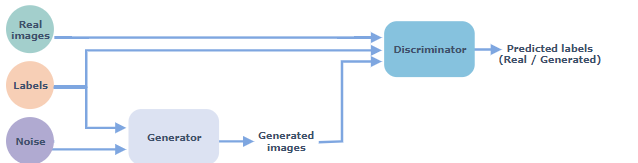
\includegraphics[width=14cm]{slike/cGAN.png}
\caption{Arhitektura cGAN mreže \citep{cGANImage}}
\label{fig:fer-logo}
\end{figure}
\textbf{}


\section{DCGAN}

Još ću se vrlo kratko osvrnuit na DCGAN arhitekturu \citep{dcgan}, modifikaciju GAN arhitekture posebno prilagođene za rad sa slikama. \textbf{Duboke konvolucije generativne suparničke mreže} \engl{deep convolutional adversarial generative networks, DCGAN} nadograđuju klasični GAN model uvodeći sljedeće izmjene:
\begin{itemize}
    \item {\large •} Slojeve sažimanja u diskriminatoru mijenja s konvolucijom s koracima \engl{strided convolution}, dok slojeve sažimanja u generatoru mijenja s konvolucijom s djelomičnim koracima \engl{ fractional-strided convolution}. Ovo omogućava mreži da sama nauči provoditi poduzorkovanje
    \item {\large •} Koristi \textit{batch} normalizaciju u generatoru i diskriminatoru
    \item {\large •} Uklanja potpuno povezane slojeve u dubljim arhitekturama
    \item {\large •} Koristi ReLU aktivacijsku funkciju u svim slojevima, osim u izlaznoj gdje koristi tangens hiperbolni
    \item {\large •} Koristi \textit{LeakyReLU} kao aktivacijsku funkciju u svim slojevima diskriminatora
\end{itemize}

\noindent Ove promjene poboljšavaju učenje, te u konačnici daju bolje rezultate u odnosu na klasični GAN. Također, autori su nakon treniranja mreže uspješno izdvojili diskriminatorski dio mreže te ga (samostalno) koristili kao klasifikator.


\section{cycleGAN}
Glavna motivacija za uvođenje arhitekture \textbf{cikličnih generativnih suparničkih mreža} \engl{cycle generative adversarial networks, cycleGAN} je problem prevođenja slika iz domene A u domenu B. Primjerice, želimo naučiti mrežu da za danu sliku livade u proljeće generira sliku iste livade ali recimo zimi. Ili na osnovu poznatog umjetničkog djela, primjerice Van Goghove \textit{Zvjezdane noći}, dobiti sliku koja izgleda kao fotografija krajolika na osnovu kojeg je djelo naslikano. Tradicionalni pristupi ovakvom problemu zahtijevaju velik broj povezanih parova slika iz domene A i domene B, odnosno za ulaznu sliku iz domene A model zahtijeva \textbf{istu} tu sliku, samo iz domene B. Konkretno na našem primjeru prevođenja slika livada u proljeće u slike, postojeći modeli zahtijevaju da im kao ulaz damo puno slika livada u proljeće, ali i u zimu. Očito je kako je u određenim situacijama vrlo nezgodno, pa čak i nemoguće doći do takvih parova (kako doći do fotografije krajolika koji je Van Gogh gledao kad je slikao \textit{Zvjezdanu noć}?)

Arhitektura cycleGAN, prvi put opisana u \citep{cycleGANOriginal}, rješava navedeni problem. U klasičnom (c)GAN pristupu, generator bi naučio mapiranje $G: X \longrightarrow Y$, gdje je X početna, a Y ciljna domena. U kombinaciji s diskriminatorom koji bi učio razliku između $y$ (originalnih ulaza) i $ \hat{y}$ (generiranih ulaza), G bi u idealnom slučaju savršeno naučio distribuciju od $Y$, te bi generirane slike bilo nemoguće raspoznati od originalnih slika. Međutim, ovo uvijek ne garantira da će originalni $x$ i generirani $y$ biti povezani na smislen način, jer postoji beskonačno mnogo mapiranja $G:X \longrightarrow Y$ koji će rezultirati savršenom distribucijom $y$. Također, kod ovakvog pristupa pojavljuje se \textit{mode collapse} problem, gdje se svi ulazni $x$ mapiraju na isti $y$, te učenje stagnira. Postoje određena rješenja ovih problema (evidentno iz postojanja pix2pix cGAN arhitekture spomenute u 4.2), no autori za rješavanje ovih problema predlažu da bi treniranje modela trebalo biti \textit{ciklički konzistentno}, odnosno da model paralelno uz učenje mapiranja $G:X \longrightarrow Y$, uči i inverzno mapiranje $F:Y \longrightarrow X$, odnosno G i F moraju biti inverzne funkcije, te ujedno i bijekcije. Tu praksi znači da ćemo u mreži imati dva generatora i dva diskriminatora. Prvi generator, G, uči mapiranje $G:X \longrightarrow Y$. Prvi diskriminator, $D_{y}$, uči razlikovati originalne slike iz skupa $X$ i slike iz $X$ koje generira G. Drugi generator, F, uči obrnuto mapiranje, $F:Y \longrightarrow X$, a drugi diskriminator, $D_{x}$, kako razlikovati originalne slike iz $Y$, te slike koje generira F. Slika 4.3 prikazuje navedenu arhitekturu.\\

\begin{figure}[htb]
\centering
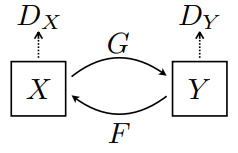
\includegraphics[width=8cm]{slike/cycleGAN1.png}
\caption{Generatori i diskriminatori cycleGAN arhitekture \citep{cycleGANOriginal}}
\label{fig:fer-logo}
\end{figure}
\textbf{}


\noindent Kako bi uspješno trenirali ovu mrežu, uvodimo nekoliko novih funkcija gubitka. Za generator G i pripadajući mu diskriminator $D_{y}$ izražavamo cilj kao:

\begin{myequation}%
\bm{\mathcal{L}_{GAN}(G,D_{y}, X, Y) = \mathbb{E}_{y \sim p_{data}(y) } [logD_{Y}(y))] + \mathbb{E}_{x \sim p_{data}(x)}[log(1-D_{Y}(G(x))]}  %
\end{myequation}

Kao i kod klasičnog GAN-a, G nastoji minimizirati ovu funkciju, dok ju D nastoji maksimizirati. Na ekvivalentan način definiramo i cilj za F i $D_{x}$:

\begin{myequation}%
\bm{\mathcal{L}_{GAN}(F,D_{x}, X, Y) = \mathbb{E}_{x \sim p_{data}(x) } [logD_{X}(x))] + \mathbb{E}_{y \sim p_{data}(y)}[log(1-D_{X}(F(y))]
}  %
\end{myequation}

Konačno, uvodimo pojam \textbf{ciklične funkcije gubitka} \engl{cycle loss}, kako bi osigurali da mapiranja G i F budu \textbf{ciklički konzistentna}. Odnosno da za svaku ulaznu sliku $x$, prolaskom kroz cijeli krug (ciklus) naše mreže, kao izlaz generatora F ponovno trebamo dobiti sliku $x$. Odnosno, želimo postići $x \longrightarrow G(x) \longrightarrow F(G(x)) = x$. Ovu relaciju zovemo \textbf{unaprijedna ciklična konzistentnost}. Također želimo postići i obrnuto, odnosno za svaku sliku iz domene $Y$, treba vrijediti $y \longrightarrow F(y) \longrightarrow G(F(y)) = y$. Model potičemo da nauči ovakvo ponašanje uvođenjem cikličke funkcije gubitka: 

\begin{myequation}%
\bm{\mathcal{L}(G,F) = \mathbb{E}_{x \sim p_{data}(x)}[||F(G(x)) -x||_{1}] + \mathbb{E}_{y \sim p_{data}(y)}[||G(F(y)) - y||_{1}]}  %
\end{myequation}

Ukupnu funkciju gubitka dobivamo zbrajanjem navedenih funkcija:

\begin{myequation}%
\bm{\mathcal{L} (G,F,D_{X},D_{Y}) = \mathcal{L}_{GAN}(G,D_{Y},X,Y) + \mathcal{L}_{GAN}(F,D_{x}, Y, X) + \lambda\mathcal{L}_{cyc}(G,F)
}  %
\end{myequation}


\noindent Na slici 4.4 vidimo neke od brojnih mogućih primjena cycleGAN arhitekture.

\begin{figure}[htb]
\hspace{-2cm}
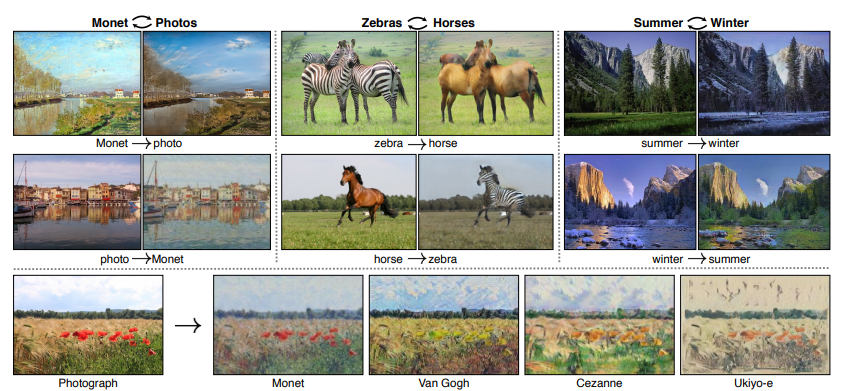
\includegraphics[width=18cm]{slike/cycleGAN2.png}
\caption{Primjene cycleGAN arhitekture \citep{cycleGANOriginal}}
\label{fig:fer-logo}
\end{figure}
\textbf{}
